\documentclass[10pt,a4paper,twoside]{article}

\usepackage[a4paper, top=18mm, bottom=18mm, left=16mm, right=16mm,
            headheight=14pt]{geometry}
\usepackage{tikz}
\usetikzlibrary{shapes.geometric,arrows.meta,positioning,fit,backgrounds,
                automata,calc,decorations.pathreplacing}
\usepackage{booktabs}
\usepackage{array}
\usepackage{xcolor}
\usepackage{colortbl}
\usepackage{enumitem}
\usepackage{multicol}
\usepackage{multirow}
\usepackage{tabularx}
\usepackage{longtable}
\usepackage{titlesec}
\usepackage{fancyhdr}
\usepackage{hyperref}
\usepackage{amsmath}
\usepackage{amssymb}
\usepackage{listings}
\usepackage{caption}
\usepackage{pdflscape}
\usepackage{makecell}

%% ── colours ────────────────────────────────────────────────────────────────
\definecolor{navyblue}{HTML}{1B2A4A}
\definecolor{steelblue}{HTML}{2E6DA4}
\definecolor{skyblue}{HTML}{BDD7EE}
\definecolor{amber}{HTML}{F4A261}
\definecolor{amberlt}{HTML}{FDE8CC}
\definecolor{teal}{HTML}{2A9D8F}
\definecolor{teallt}{HTML}{C8ECEA}
\definecolor{crimson}{HTML}{C0392B}
\definecolor{lightgray}{HTML}{F2F2F2}
\definecolor{midgray}{HTML}{CCCCCC}
\definecolor{darkgray}{HTML}{555555}

%% ── hyperref ────────────────────────────────────────────────────────────────
\hypersetup{colorlinks=true,linkcolor=steelblue,urlcolor=teal,
            citecolor=teal,pdfauthor={JESD79-5 Reference},
            pdftitle={DDR5 SDRAM Complete Reference}}

%% ── page style ──────────────────────────────────────────────────────────────
\pagestyle{fancy}
\fancyhf{}
\fancyhead[LE]{\small\textcolor{navyblue}{\textbf{DDR5 SDRAM — JESD79-5 Reference}}}
\fancyhead[RO]{\small\textcolor{crimson}{\rightmark}}
\fancyfoot[C]{\small\thepage}
\renewcommand{\headrulewidth}{0.4pt}

%% ── section style ───────────────────────────────────────────────────────────
\titleformat{\section}{\large\bfseries\color{navyblue}}{\thesection}{0.6em}{}[\vspace{-4pt}\textcolor{navyblue}{\rule{\linewidth}{0.5pt}}]
\titlespacing{\section}{0pt}{10pt}{4pt}

\titleformat{\subsection}
  {\normalsize\bfseries\color{navyblue}}{\thesubsection}{0.6em}{}
  [\vspace{-4pt}\textcolor{steelblue}{\rule{\linewidth}{0.3pt}}]
\titlespacing{\subsection}{0pt}{8pt}{2pt}

\titleformat{\subsubsection}
  {\small\bfseries\color{steelblue}}{\thesubsubsection}{0.5em}{}
\titlespacing{\subsubsection}{0pt}{5pt}{1pt}

%% ── list style ──────────────────────────────────────────────────────────────
\setlist[itemize]{itemsep=1.5pt,topsep=2pt,parsep=0pt,
                  label=\textcolor{steelblue}{$\blacktriangleright$}}
\setlist[itemize,2]{label=\textcolor{teal}{$\circ$},leftmargin=1.6em}
\setlist[description]{itemsep=1pt,font=\bfseries\color{navyblue}}

%% ── table style ─────────────────────────────────────────────────────────────
\newcommand{\thd}[1]{\cellcolor{navyblue}\textcolor{white}{\textbf{#1}}}
\newcommand{\thdm}[1]{\cellcolor{steelblue}\textcolor{white}{\small\textbf{#1}}}
\newcommand{\trow}{\rowcolor{lightgray}}
\newcommand{\talt}{\rowcolor{skyblue!30}}
\arrayrulecolor{midgray}

%% ── TikZ styles ─────────────────────────────────────────────────────────────
\tikzset{
  blk/.style={rectangle,rounded corners=3pt,draw=navyblue,fill=skyblue!40,
              minimum width=2.4cm,minimum height=0.75cm,
              font=\small\bfseries,align=center,text=navyblue},
  sblk/.style={rectangle,rounded corners=2pt,draw=teal,fill=teallt,
               minimum width=2cm,minimum height=0.6cm,
               font=\scriptsize,align=center,text=teal},
  st/.style={circle,draw=navyblue,fill=skyblue!30,minimum size=1.2cm,
             font=\scriptsize\bfseries,align=center,text=navyblue},
  arr/.style={-Stealth,thick,color=navyblue},
  rarr/.style={-Stealth,thick,color=crimson},
  tarr/.style={-Stealth,thick,color=teal},
  grp/.style={rectangle,rounded corners=5pt,draw=#1!50,fill=#1!5,
              dashed,inner sep=8pt},
}

%% ── misc ────────────────────────────────────────────────────────────────────
\captionsetup{font=small,labelfont={bf,color=navyblue},skip=4pt}
\setlength{\parskip}{2pt}
\setlength{\parindent}{0pt}

%%%%%%%%%%%%%%%%%%%%%%%%%%%%%%%%%%%%%%%%%%%%%%%%%%%%%%%%%%%%%%%%%%%%%%%%%%%%
\begin{document}

%% ── TITLE PAGE ──────────────────────────────────────────────────────────────
\begin{titlepage}
\pagecolor{navyblue}
\color{white}
\vspace*{3cm}
\begin{center}
{\fontsize{36}{44}\selectfont\bfseries DDR5 SDRAM}\\[8pt]
{\fontsize{20}{28}\selectfont Complete Reference Document}\\[16pt]
{\large\color{amber} Based on JEDEC Standard JESD79-5 (July 2020)}\\[8pt]
{\normalsize DDR5-3200 through DDR5-6400 $\;\cdot\;$ LPDDR5 Cross-reference
$\;\cdot\;$ DFI 5.2 Mapping}
\vfill
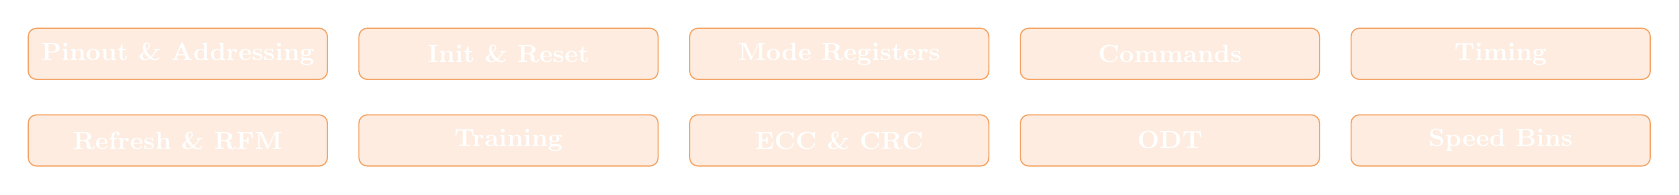
\begin{tikzpicture}
  \foreach \i/\lbl in {
    0/Pinout \& Addressing,
    1/Init \& Reset,
    2/Mode Registers,
    3/Commands,
    4/Timing,
    5/Refresh \& RFM,
    6/Training,
    7/ECC \& CRC,
    8/ODT,
    9/Speed Bins}{
    \node[rectangle,rounded corners=3pt,draw=amber,fill=amber!20,
          text=white,minimum width=3.8cm,minimum height=0.65cm,
          font=\small\bfseries,align=center]
      at ({mod(\i,5)*4.2cm - 8.4cm},{-floor(\i/5)*1.1cm}) {\lbl};
  }
\end{tikzpicture}
\vfill
{\small\color{midgray} Compiled from JESD79-5 $\cdot$ 496 pages $\cdot$
Covers SDRAM architecture, electrical, timing, MR0--MR63+DFE, all commands,
speed bins 3200--6400}
\end{center}
\end{titlepage}
\pagecolor{white}\color{black}

%% ── TOC ─────────────────────────────────────────────────────────────────────
\tableofcontents
\clearpage

%%%%%%%%%%%%%%%%%%%%%%%%%%%%%%%%%%%%%%%%%%%%%%%%%%%%%%%%%%%%%%%%%%%%%%%%%%%%
\section{DDR5 Architecture Overview}
%%%%%%%%%%%%%%%%%%%%%%%%%%%%%%%%%%%%%%%%%%%%%%%%%%%%%%%%%%%%%%%%%%%%%%%%%%%%

\subsection{Key Architectural Changes vs DDR4}

\begin{itemize}
  \item \textbf{16n prefetch}: BL16 native (vs 8n in DDR4); optional BL8 (BC8) and BL32
  \item \textbf{Split channel}: one DIMM = two independent 32-bit sub-channels (A \& B), each with own DQS
  \item \textbf{On-die ECC}: SEC (Single-Error Correction) mandatory; no separate ECC DRAM needed for x4/x8
  \item \textbf{Bank groups}: x4/x8: 8 BG $\times$ 4 banks = 32 banks (8\,Gb) or 32 banks (16\,Gb+); x16: 4 BG $\times$ 4 = 16 banks
  \item \textbf{Command bus}: 14-bit CA bus replaces traditional RAS/CAS/WE; 2-cycle command encoding
  \item \textbf{New commands}: MPC, VrefCA, VrefCS; RFMab/RFMsb; WR\_PARTIAL; BL32
  \item \textbf{PMIC on DIMM}: Power management on-module; VDD = 1.1\,V (vs 1.2\,V DDR4)
  \item \textbf{CRC}: Mandatory write CRC; read CRC optional
  \item \textbf{DFE}: Decision Feedback Equalization in DRAM Rx
  \item \textbf{Refresh Management (RFM)}: Rowhammer mitigation built into spec
\end{itemize}

\subsection{Signal Comparison: DDR4 vs DDR5}

\begin{center}
\begin{tabularx}{\linewidth}{@{} l X X @{}}
\toprule
\thd{Signal} & \thd{DDR4} & \thd{DDR5} \\
\midrule
\trow Command bus & RAS\_n/CAS\_n/WE\_n/BA/A[13:0] & CA[13:0] + CS\_n (2-cycle) \\
\talt Data width & x4/x8/x16 & x4/x8/x16 (per sub-channel x4/x8) \\
\trow Prefetch & 8n & 16n (BL16 default) \\
\talt Clock & CK\_t/CK\_c & CK\_t/CK\_c \\
\trow DQS & DQS\_t/DQS\_c per byte & DQS\_t/DQS\_c per byte \\
\talt Alert & ALERT\_n & ALERT\_n \\
\trow ZQ & ZQ pin, ZQCL/ZQCS via MRS & ZQ pin, ZQCAL via MPC \\
\talt Power & VDD=1.2V, VDDQ=1.2V, VPP=2.5V & VDD=1.1V, VDDQ=1.1V, VPP=1.8V \\
\trow ODT & Dynamic ODT via MRS & Dynamic ODT via MR + CA\_ODT strap \\
\talt Reset & RESET\_n & RESET\_n \\
\bottomrule
\end{tabularx}
\end{center}

%%%%%%%%%%%%%%%%%%%%%%%%%%%%%%%%%%%%%%%%%%%%%%%%%%%%%%%%%%%%%%%%%%%%%%%%%%%%
\section{Package, Pinout \& Addressing}
%%%%%%%%%%%%%%%%%%%%%%%%%%%%%%%%%%%%%%%%%%%%%%%%%%%%%%%%%%%%%%%%%%%%%%%%%%%%

\subsection{Package Specifications}

\begin{itemize}
  \item \textbf{Package}: MO-210 BGA, ball pitch 0.8\,mm $\times$ 0.8\,mm
  \item x4/x8: 13 electrical rows, 6 electrical columns (2 sets of 3)
  \item 3 depopulated columns between electrical columns
\end{itemize}

\subsection{Pinout Description}

\begin{center}
\begin{tabularx}{\linewidth}{@{} l l X @{}}
\toprule
\thd{Pin} & \thd{Type} & \thd{Description} \\
\midrule
\trow CK\_t, CK\_c & Input & Differential clock. All inputs sampled on CK\_t rising edge \\
\talt CA[13:0] & Input & 14-bit command/address bus. Latched on both CK edges for 2-cycle cmds \\
\trow CS\_n & Input & Chip Select. Active LOW. Selects device for command reception \\
\talt DQ[3:0/7:0/15:0] & I/O & Data bus. Width depends on device configuration \\
\trow DQS\_t, DQS\_c & I/O & Differential data strobe. Source-synchronous. 1 per byte \\
\talt DM\_n/TDQS & I/O & Data mask (write) / Termination DQS (x8). MR-controlled \\
\trow RESET\_n & Input & Async reset. Active LOW. Initializes all internal logic \\
\talt ALERT\_n & Output & Open-drain alert: CRC error, CA parity error, temp alert \\
\trow ZQ & Ref & External ZQ calibration resistor (240\,$\Omega$ $\pm$1\%) \\
\talt VDD & PWR & Core supply 1.1\,V nom \\
\trow VDDQ & PWR & I/O supply 1.1\,V nom \\
\talt VPP & PWR & Activating power supply 1.8\,V \\
\trow VSS/VSSQ & GND & Core/IO ground \\
\talt LBDQ, LBDQS & I/O & Loopback data/strobe (optional) \\
\bottomrule
\end{tabularx}
\end{center}

\subsection{Addressing Tables}

\subsubsection{8\,Gb Devices}
\begin{center}
\begin{tabularx}{\linewidth}{@{} l l l l l l l @{}}
\toprule
\thd{Config} & \thd{BG} & \thd{BA} & \thd{BG/Banks} & \thd{Row} & \thd{Col} & \thd{Page} \\
\midrule
\trow 8\,Gb x4 & BG0--2 & BA0--1 & 8/2/16 & R0--R16 & C0--C10 & 1\,KB \\
\talt 8\,Gb x8 & BG0--2 & BA0--1 & 8/2/16 & R0--R16 & C0--C9  & 1\,KB \\
\trow 8\,Gb x16 & BG0--1 & BA0--1 & 4/2/8  & R0--R16 & C0--C9  & 2\,KB \\
\bottomrule
\end{tabularx}
\end{center}

\subsubsection{16\,Gb Devices (and higher: 32\,Gb, 64\,Gb)}
\begin{center}
\begin{tabularx}{\linewidth}{@{} l l l l l l l @{}}
\toprule
\thd{Config} & \thd{BG} & \thd{BA} & \thd{BG/Banks/Total} & \thd{Row} & \thd{Col} & \thd{Page} \\
\midrule
\trow 16\,Gb x4 & BG0--2 & BA0--1 & 8/4/32 & R0--R16 & C0--C10 & 1\,KB \\
\talt 16\,Gb x8 & BG0--2 & BA0--1 & 8/4/32 & R0--R16 & C0--C9  & 1\,KB \\
\trow 16\,Gb x16 & BG0--1 & BA0--1 & 4/4/16 & R0--R16 & C0--C9 & 2\,KB \\
\midrule
\trow 32\,Gb x4 & BG0--2 & BA0--1 & 8/4/32 & R0--R16 & C0--C10 & 1\,KB \\
\talt 32\,Gb x8 & BG0--2 & BA0--1 & 8/4/32 & R0--R16 & C0--C9  & 1\,KB \\
\trow 32\,Gb x16 & BG0--1 & BA0--1 & 4/4/16 & R0--R16 & C0--C9 & 2\,KB \\
\midrule
\trow 64\,Gb x4 & BG0--2 & BA0--1 & 8/4/32 & R0--R17 & C0--C10 & 1\,KB \\
\talt 64\,Gb x8 & BG0--2 & BA0--1 & 8/4/32 & R0--R17 & C0--C9  & 1\,KB \\
\trow 64\,Gb x16 & BG0--1 & BA0--1 & 4/4/16 & R0--R17 & C0--C9 & 2\,KB \\
\bottomrule
\end{tabularx}
\end{center}

\textit{3DS (3D Stacked):} CID[3:0] selects die in stack. Max stack: 8H (x4/x8) or 4H (x16).

%%%%%%%%%%%%%%%%%%%%%%%%%%%%%%%%%%%%%%%%%%%%%%%%%%%%%%%%%%%%%%%%%%%%%%%%%%%%
\section{Reset and Initialization}
%%%%%%%%%%%%%%%%%%%%%%%%%%%%%%%%%%%%%%%%%%%%%%%%%%%%%%%%%%%%%%%%%%%%%%%%%%%%

\subsection{Power-Up Initialization Sequence}

Steps (ref: JESD79-5 \S3.3.1):
\begin{enumerate}[itemsep=2pt]
  \item Apply VPP before or simultaneously with VDD/VDDQ
  \item RESET\_n held LOW for $\geq$ tINIT1 (200\,$\mu$s) after voltage ramp completes
  \item CS\_n pulled LOW at least tINIT2 (10\,ns) before RESET\_n HIGH
  \item After RESET\_n HIGH: CS\_n stays LOW for $\geq$ tINIT3 (4\,ms)
  \item DRAM registers EXIT on CS\_n: wait tINIT4 (2\,$\mu$s minimum)
  \item Issue $\geq$ 3 NOP after CS\_n HIGH (tINIT5)
  \item Stable clock required: tCKSRX before any command
  \item Issue \textbf{MPC DLL Reset}
  \item Issue \textbf{MPC ZQCAL Start} $\rightarrow$ wait tZQCAL
  \item Issue \textbf{MPC ZQCAL Latch} $\rightarrow$ wait tZQLAT
  \item Program MRs (MR0, MR2, MR3, MR4, MR5, MR6, MR8, MR32--35, MR34--35)
  \item Perform training (WL, read gate, read/write DQ, CA, CS, VREF)
\end{enumerate}

\subsection{Initialization Timing Parameters}

\begin{center}
\begin{tabularx}{0.85\linewidth}{@{} l l r r l @{}}
\toprule
\thd{Parameter} & \thd{Symbol} & \thd{Min} & \thd{Max} & \thd{Unit} \\
\midrule
\trow Max voltage ramp time & tINIT0 & -- & 20 & ms \\
\talt RESET\_n LOW after voltage ramp & tINIT1 & 200 & -- & $\mu$s \\
\trow CS\_n LOW before RESET\_n HIGH & tINIT2 & 10 & -- & ns \\
\talt CS\_n LOW after RESET\_n HIGH & tINIT3 & 4 & -- & ms \\
\trow DRAM EXIT registration & tINIT4 & 2 & -- & $\mu$s \\
\talt NOP cycles after CS HIGH & tINIT5 & 3 & -- & nCK \\
\trow Exit Reset to first config cmd & tXPR & tXS & -- & -- \\
\talt Stable clock before command & tCKSRX & See SR tables & -- & -- \\
\trow MR write period & tMRW & max(5\,ns,~8\,nCK) & -- & nCK \\
\talt MR read period & tMRR & max(14\,ns,~16\,nCK) & -- & nCK \\
\trow MR set delay & tMRD & max(14\,ns,~16\,nCK) & -- & nCK \\
\bottomrule
\end{tabularx}
\end{center}

\subsection{Init FSM State Diagram}

\vspace{4pt}
\begin{center}
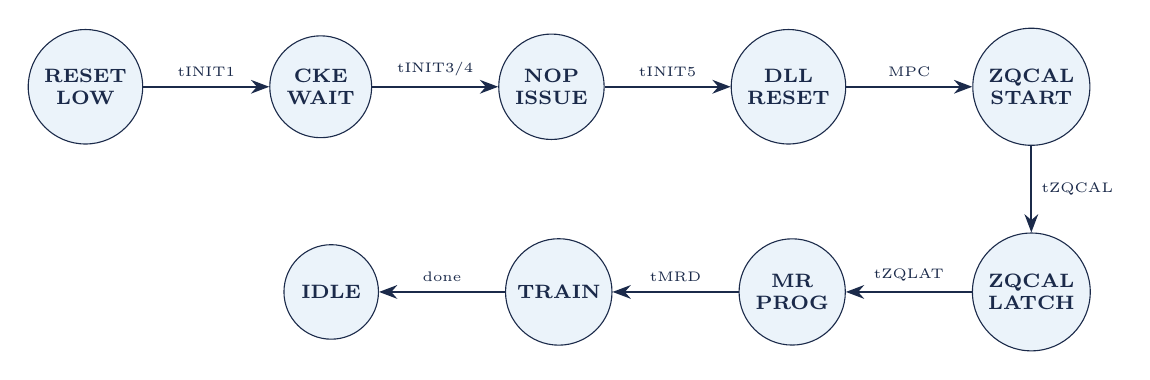
\begin{tikzpicture}[node distance=0.9cm and 1.6cm, font=\scriptsize]
  \node[st] (rst)  {RESET\\LOW};
  \node[st, right=of rst] (cke)  {CKE\\WAIT};
  \node[st, right=of cke] (nop)  {NOP\\ISSUE};
  \node[st, right=of nop] (dll)  {DLL\\RESET};
  \node[st, right=of dll] (zqcs) {ZQCAL\\START};
  \node[st, below=1.1cm of zqcs] (zqcl){ZQCAL\\LATCH};
  \node[st, left=of zqcl] (mr)   {MR\\PROG};
  \node[st, left=of mr]   (trn)  {TRAIN};
  \node[st, left=of trn]  (idle) {IDLE};

  \draw[arr] (rst)  -- node[above,font=\tiny]{tINIT1} (cke);
  \draw[arr] (cke)  -- node[above,font=\tiny]{tINIT3/4} (nop);
  \draw[arr] (nop)  -- node[above,font=\tiny]{tINIT5} (dll);
  \draw[arr] (dll)  -- node[above,font=\tiny]{MPC} (zqcs);
  \draw[arr] (zqcs) -- node[right,font=\tiny]{tZQCAL} (zqcl);
  \draw[arr] (zqcl) -- node[above,font=\tiny]{tZQLAT} (mr);
  \draw[arr] (mr)   -- node[above,font=\tiny]{tMRD} (trn);
  \draw[arr] (trn)  -- node[above,font=\tiny]{done} (idle);
\end{tikzpicture}
\end{center}

\subsection{MR Default Settings at Power-Up}

\begin{center}
\begin{tabularx}{\linewidth}{@{} l l l X @{}}
\toprule
\thd{Item} & \thd{MR} & \thd{Default} & \thd{Description} \\
\midrule
\trow Burst Length & MR0 OP[1:0] & 00B & BL16 \\
\talt Read Latency & MR0 OP[6:2] & 00010B & RL=26 @ DDR5-3200 \\
\trow Write Recovery & MR6 OP[3:0] & 0000B & tWR=48\,nCK @ 3200 or 30\,ns \\
\talt tRTP & MR6 OP[7:4] & 0000B & 12\,nCK @ 3200 or 7.5\,ns \\
\trow VrefDQ & MR10 & 0010 1101B & 75\% VDDQ \\
\talt VrefCA & MR11 & 0010 1101B & 75\% VDDQ \\
\trow VrefCS & MR12 & 0010 1101B & 75\% VDDQ \\
\talt ECS threshold & MR15 & 011B & 256 errors \\
\trow PPR & MR23 OP[1:0] & 00B & hPPR \& sPPR disabled \\
\talt CK ODT & MR32 OP[2:0] & strap & Group A: RTT\_OFF; Group B: 40\,$\Omega$ \\
\trow CS ODT & MR32 OP[5:3] & strap & Group A: RTT\_OFF; Group B: 40\,$\Omega$ \\
\talt CA ODT & MR33 OP[2:0] & strap & Group A: RTT\_OFF; Group B: 80\,$\Omega$ \\
\trow RTT\_WR & MR34 OP[5:3] & 001B & 240\,$\Omega$ \\
\talt RTT\_NOM\_WR & MR35 OP[2:0] & 011B & 80\,$\Omega$ \\
\bottomrule
\end{tabularx}
\end{center}

%%%%%%%%%%%%%%%%%%%%%%%%%%%%%%%%%%%%%%%%%%%%%%%%%%%%%%%%%%%%%%%%%%%%%%%%%%%%
\section{Mode Registers}
%%%%%%%%%%%%%%%%%%%%%%%%%%%%%%%%%%%%%%%%%%%%%%%%%%%%%%%%%%%%%%%%%%%%%%%%%%%%

\subsection{MR Addressing Scheme}

DDR5 uses LPDDR-style MR protocol: 8-bit \textbf{MRA} (Mode Register Address) + 8-bit \textbf{OP} (operand payload).
Commands: \textbf{MRW} (write) and \textbf{MRR} (read), encoded on CA bus.
Up to 256 addressable byte-wide registers (MR0--MR255).

\subsection{MR0 --- Burst Length / Read Latency}

\begin{center}
\begin{tabularx}{\linewidth}{@{} l l l X @{}}
\toprule
\thd{Bits} & \thd{R/W} & \thd{Field} & \thd{Encoding} \\
\midrule
\trow OP[1:0] & R/W & Burst Length &
  00B: BL16 (default) $|$ 01B: BC8 (OTF) $|$ 10B: BC8 fixed $|$ 11B: BL32 \\
\talt OP[6:2] & R/W & CAS Latency (RL) &
  00000B: RFU $|$ 00001B: CL22 $|$ 00010B: CL26 $|$ \ldots see Table 25 \\
\trow OP[7] & RFU & -- & Reserved \\
\bottomrule
\end{tabularx}
\end{center}

\textbf{CL encoding (OP[6:2]):} 00010B=26, 00011B=28, 00100B=30, 00101B=32, 00110B=34, 00111B=36,
01000B=38, 01001B=40, 01010B=42, 01011B=44, 01100B=46, 01101B=48, 01110B=50, 01111B=52,
10000B=54, 10001B=56, 10010B=58, 10011B=60, 10100B=62, 10101B=CL22 (bin A only).

\subsection{MR1 --- Drive Impedance / ODT}

\begin{center}
\begin{tabularx}{\linewidth}{@{} l l l X @{}}
\toprule
\thd{Bits} & \thd{R/W} & \thd{Field} & \thd{Encoding} \\
\midrule
\trow OP[2:0] & R/W & Pull-Down Drive Impedance &
  000B: RFU $|$ 001B: 34\,$\Omega$ (RZQ/7) $|$ 010B: 40\,$\Omega$ (RZQ/6) $|$
  011B: 48\,$\Omega$ (RZQ/5) $|$ 100B: 60\,$\Omega$ $|$ 101B: 80\,$\Omega$ $|$ 110--111B: RFU \\
\talt OP[5:3] & R/W & Pull-Up Drive Impedance & Same encoding as OP[2:0] \\
\trow OP[6] & R/W & CS Assertion Duration &
  0B: 1-cycle $|$ 1B: 2-cycle \\
\talt OP[7] & R/W & Internal Write Timing &
  0B: Disabled (default) $|$ 1B: Enabled \\
\bottomrule
\end{tabularx}
\end{center}

\subsection{MR2 --- Functional Modes}

\begin{center}
\begin{tabularx}{\linewidth}{@{} l l l X @{}}
\toprule
\thd{Bits} & \thd{R/W} & \thd{Field} & \thd{Encoding} \\
\midrule
\trow OP[1:0] & R/W & Max Power Saving Mode (MPSM) & 00B: disable $|$ 01B: MPSM $|$ others: RFU \\
\talt OP[2] & R/W & Device 15 MPSM & 0B: all devices $|$ 1B: device 15 only \\
\trow OP[3] & R/W & 2N Mode & 0B: 1N $|$ 1B: 2N \\
\talt OP[4] & R/W & Read Preamble Training & 0B: disable $|$ 1B: enable \\
\trow OP[5] & R/W & Write Leveling Training & 0B: disable $|$ 1B: enable \\
\talt OP[6] & R/W & Reserved & -- \\
\trow OP[7] & R/W & Internal Write Timing & 0B: disable $|$ 1B: enable \\
\bottomrule
\end{tabularx}
\end{center}

\subsection{MR3 --- DQS Write Leveling Alignment}

\begin{center}
\begin{tabularx}{\linewidth}{@{} l l l X @{}}
\toprule
\thd{Bits} & \thd{R/W} & \thd{Field} & \thd{Encoding} \\
\midrule
\trow OP[3:0] & R/W & WL Cycle Alignment Lower Byte &
  0000B: 0\,tCK (def) $|$ 0001B: $-1$\,tCK $|$ \ldots $|$ 0110B: $-6$\,tCK (opt up to $-15$) \\
\talt OP[7:4] & R/W & WL Cycle Alignment Upper Byte (x16) & Same encoding; x16 only \\
\bottomrule
\end{tabularx}
\end{center}

\subsection{MR4 --- Refresh Settings}

\begin{center}
\begin{tabularx}{\linewidth}{@{} l l l X @{}}
\toprule
\thd{Bits} & \thd{R/W} & \thd{Field} & \thd{Encoding} \\
\midrule
\trow OP[2:0] & R (SR) & Refresh Rate &
  001B: 1$\times$ ($<$80°C) $|$ 010B: 1$\times$ (80--85°C) $|$
  011B: 2$\times$ (85--90°C) $|$ 100B: 2$\times$ (90--95°C) $|$ 101B: 2$\times$ ($>$95°C) \\
\talt OP[3] & SR/W & Refresh Interval Rate Indicator &
  0B: not implemented $|$ 1B: implemented \\
\trow OP[4] & R/W & Refresh tRFC Mode &
  0B: tRFC normal $|$ 1B: tRFC Fine Granularity (FGR) \\
\talt OP[6:5] & RFU & -- & -- \\
\trow OP[7] & R & TUF (Temperature Update Flag) &
  0B: no change $|$ 1B: change since last MR4 read \\
\bottomrule
\end{tabularx}
\end{center}

\subsection{MR5 --- ODT / DM}

\begin{center}
\begin{tabularx}{\linewidth}{@{} l l l X @{}}
\toprule
\thd{Bits} & \thd{R/W} & \thd{Field} & \thd{Encoding} \\
\midrule
\trow OP[2:0] & R/W & RTT\_PARK &
  000B: off $|$ 001B: 240\,$\Omega$ $|$ 010B: 120\,$\Omega$ $|$ 011B: 80\,$\Omega$ $|$
  100B: 60\,$\Omega$ $|$ 101B: 48\,$\Omega$ $|$ 110B: 40\,$\Omega$ $|$ 111B: 34\,$\Omega$ \\
\talt OP[5] & R/W & DM Enable & 0B: disable $|$ 1B: enable \\
\trow OP[6] & R/W & TDQS Enable (x8 only) & 0B: disable $|$ 1B: enable \\
\talt OP[7] & R/W & Data Output Disable & 0B: normal $|$ 1B: tri-state DQ/DQS \\
\bottomrule
\end{tabularx}
\end{center}

\subsection{MR6 --- tWR / tRTP}

\begin{center}
\begin{tabularx}{\linewidth}{@{} l l l X @{}}
\toprule
\thd{Bits} & \thd{R/W} & \thd{Field} & \thd{Encoding} \\
\midrule
\trow OP[3:0] & R/W & tWR &
  0000B: 48\,nCK/30\,ns $|$ 0001B: 56\,nCK/35\,ns $|$ 0010B: 64\,nCK/40\,ns $|$
  0011B: 72\,nCK/45\,ns $|$ 0100B: 80\,nCK/50\,ns $|$ 0101B: 96\,nCK/60\,ns $|$
  0110B: 112\,nCK $|$ 0111B: 128\,nCK $|$ 1000B: 144\,nCK $|$ 1001B: 160\,nCK $|$
  1010B: 192\,nCK $|$ 1011B: 224\,nCK $|$ 1100B: 256\,nCK \\
\talt OP[7:4] & R/W & tRTP &
  0000B: 12\,nCK/7.5\,ns $|$ 0001B: 16\,nCK/10\,ns $|$ 0010B: 20\,nCK/12.5\,ns $|$
  others: see Table \\
\bottomrule
\end{tabularx}
\end{center}

\subsection{MR8 --- Burst Length / Training / CRC}

\begin{center}
\begin{tabularx}{\linewidth}{@{} l l l X @{}}
\toprule
\thd{Bits} & \thd{R/W} & \thd{Field} & \thd{Encoding} \\
\midrule
\trow OP[1:0] & R/W & Burst Length & 00B: BL16 $|$ 01B: BC8 OTF $|$ 10B: BC8 fixed $|$ 11B: BL32 \\
\talt OP[2] & R/W & Read Preamble & 0B: 2\,tCK $|$ 1B: 4\,tCK \\
\trow OP[3] & R/W & Write Preamble & 0B: 2\,tCK $|$ 1B: 4\,tCK \\
\talt OP[4] & R/W & Read Postamble & 0B: 0.5\,tCK $|$ 1B: 1.5\,tCK \\
\trow OP[5] & R/W & Write Postamble & 0B: 0.5\,tCK $|$ 1B: 1.5\,tCK \\
\talt OP[6] & R/W & Write CRC Enable & 0B: disable $|$ 1B: enable \\
\trow OP[7] & R/W & Read CRC Enable & 0B: disable $|$ 1B: enable \\
\bottomrule
\end{tabularx}
\end{center}

\subsection{MR10, MR11, MR12 --- VREF Settings}

\begin{center}
\begin{tabularx}{\linewidth}{@{} l l X @{}}
\toprule
\thd{MR} & \thd{Bits} & \thd{Function} \\
\midrule
\trow MR10 & OP[7:0] & VrefDQ global calibration value. Range: 35.0--97.5\% VDDQ in 0.5\% steps. Default: 0x2D = 75\% \\
\talt MR11 & OP[7:0] & VrefCA global calibration value. 75\% default \\
\trow MR12 & OP[7:0] & VrefCS global calibration value. 75\% default \\
\bottomrule
\end{tabularx}
\end{center}

Per-pin VrefDQ trims available in MR118, MR126, MR134, \ldots MR254 (OP[7:4]),
$\pm$3 steps max. Combined global + per-pin must stay within 35.0--97.5\%.

\subsection{MR13 --- RFU (reserved)}

\subsection{MR14 --- ECS (ECC Scrub) Control}

\begin{itemize}
  \item OP[1:0]: ECS mode $-$ 00B: disabled $|$ 01B: ECS during self-refresh $|$ 10B: ECS during normal operation
  \item OP[4:2]: ECS interval (tECSint)
  \item OP[7:5]: Transparency mode selector
\end{itemize}

\subsection{MR15 --- ECS Error Threshold}

\texttt{OP[2:0]}: ECS Error Threshold Count (ETC):
000B=1, 001B=4, 010B=16, 011B=256 (default), 100B=1024, 101B=4096, 110B=16384, 111B=65536.

\subsection{MR16--MR21 --- ECC Error Logging}

\begin{itemize}
  \item MR16--MR19: Row address of max-error row (R[17:0] across 4 bytes)
  \item MR20: Number of rows/code words with errors per die
  \item MR21: RFU
\end{itemize}

\subsection{MR23 --- Post Package Repair (PPR)}

\texttt{OP[1:0]}: 00B = hPPR/sPPR disabled (default) $|$ 01B = hPPR $|$ 10B = sPPR $|$ 11B = RFU

\subsection{MR24 --- PPR Guard Key}

Guard key encoding prevents accidental PPR: specific OP values required before PPR activation.

\subsection{MR32 --- CK/CS ODT Settings}

\begin{center}
\begin{tabularx}{\linewidth}{@{} l l l X @{}}
\toprule
\thd{Bits} & \thd{R/W} & \thd{Field} & \thd{Encoding} \\
\midrule
\trow OP[2:0] & R/W & CK ODT &
  000B: RTT\_OFF $|$ 001B: 240\,$\Omega$ $|$ 010B: 120\,$\Omega$ $|$ 011B: 80\,$\Omega$ $|$
  100B: 60\,$\Omega$ $|$ 101B: 48\,$\Omega$ $|$ 110B: 40\,$\Omega$ $|$ 111B: 34\,$\Omega$ \\
\talt OP[5:3] & R/W & CS ODT & Same encoding \\
\trow OP[7:6] & RFU & -- & -- \\
\bottomrule
\end{tabularx}
\end{center}

\subsection{MR33--MR35 --- CA/DQS/RTT Settings}

\begin{center}
\begin{tabularx}{\linewidth}{@{} l l X @{}}
\toprule
\thd{MR} & \thd{Bits} & \thd{Function} \\
\midrule
\trow MR33 & OP[2:0] & CA ODT (Group A: RTT\_OFF, Group B: 80\,$\Omega$ default) \\
\talt MR33 & OP[5:3] & DQS\_RTT\_PARK (000B: RTT\_OFF default) \\
\trow MR34 & OP[2:0] & RTT\_PARK (000B: RTT\_OFF default) \\
\talt MR34 & OP[5:3] & RTT\_WR (001B: 240\,$\Omega$ default) \\
\trow MR35 & OP[2:0] & RTT\_NOM\_WR (011B: 80\,$\Omega$ default) \\
\talt MR35 & OP[5:3] & RTT\_NOM\_RD (011B: 80\,$\Omega$ default) \\
\bottomrule
\end{tabularx}
\end{center}

\textbf{RTT encoding (all RTT fields):}
000B=RTT\_OFF, 001B=240\,$\Omega$, 010B=120\,$\Omega$, 011B=80\,$\Omega$,
100B=60\,$\Omega$, 101B=48\,$\Omega$, 110B=40\,$\Omega$, 111B=34\,$\Omega$

\subsection{MR58 --- Refresh Management (RFM)}

\begin{center}
\begin{tabularx}{\linewidth}{@{} l l X @{}}
\toprule
\thd{Bits} & \thd{R/W} & \thd{Encoding} \\
\midrule
\trow OP[0] & R & 0B: RFM not required $|$ 1B: RFM required \\
\talt OP[4:1] & R & RAAIMT (Initial Management Threshold): values 0100B=32, 0101B=40, \ldots \\
\trow OP[7:5] & R & RAAMMT (Maximum Management Threshold) \\
\bottomrule
\end{tabularx}
\end{center}

\subsection{MR61 --- Package Output Driver Test Mode}

Test mode for DRAM package characterization. OP[4:0] selects test pin.
Disabled = 00000B (default).

\subsection{MR63 --- DRAM Scratch Pad}

Read/write scratch register. Used by host controller to read RCD Control Words.
Any value valid; no function in DRAM itself.

\subsection{MR70--MR255 --- DFE, Per-Bit DCA \& VrefDQ}

Organized by DQ bit: DQL0 at MR128 (MA=0x80), DQL1 at MR136, \ldots DQU7 at MR248.
Each group of 8 MRs covers: DFE tap coefficients, per-bit duty cycle adjuster (DCA), per-bit VrefDQ offset.
MA[6:3] directly maps to DQ bit; MA[2:0] selects function within that DQ group.

%%%%%%%%%%%%%%%%%%%%%%%%%%%%%%%%%%%%%%%%%%%%%%%%%%%%%%%%%%%%%%%%%%%%%%%%%%%%
\section{Command Set}
%%%%%%%%%%%%%%%%%%%%%%%%%%%%%%%%%%%%%%%%%%%%%%%%%%%%%%%%%%%%%%%%%%%%%%%%%%%%

\subsection{Command Encoding Overview}

DDR5 uses a 2-cycle command protocol on CA[13:0] + CS\_n:
\begin{itemize}
  \item \textbf{Cycle 1}: CS\_n LOW + CA[13:0] encodes command type + upper address/data
  \item \textbf{Cycle 2}: CS\_n LOW or HIGH + CA[13:0] encodes lower address/data
  \item Commands decoded from CA[6:0] pattern on cycle 1
  \item \textbf{DES} (deselect): CS\_n HIGH = no operation
\end{itemize}

\subsection{Command Truth Table}

\begin{center}
\begin{tabularx}{\linewidth}{@{} l l l X @{}}
\toprule
\thd{Command} & \thd{Abbr} & \thd{CS\_n C1} & \thd{CA[13:0] C1 Key Bits / Function} \\
\midrule
\trow Deselect & DES & H & Any --- no command registered \\
\talt Activate & ACT & L & CA[6]=L, CA[5]=L, CA[4:0]=bank/BG; C2: row address \\
\trow Read & RD & L & CA[6]=L, CA[5]=H, CA[4]=L; AP, BG, BA, COL \\
\talt Read w/ AP & RD/A & L & RD + CA[10]=H (auto-precharge) \\
\trow Write & WR & L & CA[6]=H, CA[5]=L, CA[4]=L; AP, BG, BA, COL, WR\_PARTIAL \\
\talt Write w/ AP & WR/A & L & WR + CA[10]=H \\
\trow Precharge (per bank) & PRE(pb) & L & CA[5:4]=01; CA[10]=L; BG, BA \\
\talt Precharge All & PRE(ab) & L & CA[5:4]=01; CA[10]=H \\
\trow Refresh All Banks & REFab & L & CA[6:4]=001 \\
\talt Refresh Same Bank & REFsb & L & CA[6:4]=010; BA[1:0] \\
\trow Refresh Mgmt All & RFMab & L & CA encoding per Table \\
\talt Refresh Mgmt Same Bank & RFMsb & L & BA-specific \\
\trow Self Refresh Entry & SRE & L & CS pattern per Table \\
\talt Self Refresh Exit & SRX & L & Requires tCKSRX stable clock before \\
\trow Mode Register Write & MRW & L & CA[6:4]=011; C2: MRA[7:0] + OP[7:0] \\
\talt Mode Register Read & MRR & L & CA[6:4]=100; C2: MRA[7:0]; DQ returns data \\
\trow MPC (Multi-Purpose Cmd) & MPC & L & CA[13:7]=specific pattern; OP[7:0] = opcode \\
\talt VrefCA Command & VrefCA & L & Dedicated CA encoding; OP sets VREF \\
\trow VrefCS Command & VrefCS & L & Dedicated CS encoding; OP sets VREF \\
\talt Write Pattern & WRP & L & MPC opcode 0000 0001 \\
\bottomrule
\end{tabularx}
\end{center}

\subsection{ACTIVATE Command}

Opens a row in a bank for subsequent RD/WR.
\begin{itemize}
  \item BG[2:0] (x4/x8) or BG[1:0] (x16): selects bank group
  \item BA[1:0]: selects bank within group
  \item R[17:0]: row address (C1+C2 combined)
  \item 3DS: CID[3:0] selects die in stack
  \item Bank-to-bank ACT timing: \textbf{tRRD\_S} (different BG) or \textbf{tRRD\_L} (same BG)
  \item Max 4 ACTs within tFAW window
\end{itemize}

\subsection{READ / WRITE Commands}

\begin{itemize}
  \item CAS issued tRCD after ACT
  \item Read latency: \textbf{RL} = CL (set in MR0)
  \item Write latency: \textbf{WL} = CL$-$2 (CWL = CL$-$2, fixed relationship in DDR5)
  \item Data transfer: 16 UI per burst (BL16); DQ toggled on both DQS edges
  \item \textbf{AP} (CA10=H): auto-precharge after burst completes
  \item \textbf{WR\_PARTIAL}: enables DM-masked partial writes; triggers internal RMW
  \item CAS-to-CAS: tCCD\_L (same BG), tCCD\_S (diff BG); tCCD\_L\_WR for WR-to-WR same BG
\end{itemize}

\subsection{MPC Opcode Table (Key Opcodes)}

\begin{center}
\begin{tabularx}{0.88\linewidth}{@{} l l X @{}}
\toprule
\thd{OP[7:0]} & \thd{MPC Command} & \thd{Description} \\
\midrule
\trow 0000 0000 & ZQCALstart & Initiates ZQ calibration start \\
\talt 0000 0001 & ZQCALlatch & Latches ZQ calibration result \\
\trow 0000 0010 & DLL Reset & Resets DLL \\
\talt 0000 0011 & Write Pattern & Puts device in write pattern mode \\
\trow 0000 0100 & RTP Reset & Resets read training pattern \\
\talt 0000 0101 & RTP Start & Starts read training pattern output \\
\trow 0000 0110 & RTP Stop & Stops read training pattern \\
\talt 0001 0000 & CATraining & Enables CA training mode \\
\trow 0001 0001 & CSTraining & Enables CS training mode \\
\talt 0001 0010 & WLTraining & Enables write leveling \\
\trow 0001 0011 & Preamble Training & Enables preamble training mode \\
\talt 0001 0100 & Connectivity Test & Enters connectivity test (CT) mode \\
\trow 0001 0101 & DQS Oscillator Start & Starts DQS interval oscillator \\
\talt 0001 0110 & DQS Oscillator Stop & Stops DQS interval oscillator \\
\bottomrule
\end{tabularx}
\end{center}

%%%%%%%%%%%%%%%%%%%%%%%%%%%%%%%%%%%%%%%%%%%%%%%%%%%%%%%%%%%%%%%%%%%%%%%%%%%%
\section{Timing Parameters}
%%%%%%%%%%%%%%%%%%%%%%%%%%%%%%%%%%%%%%%%%%%%%%%%%%%%%%%%%%%%%%%%%%%%%%%%%%%%

\subsection{Key Timing Definitions}

\begin{center}
\begin{tabularx}{\linewidth}{@{} l l X @{}}
\toprule
\thd{Symbol} & \thd{Name} & \thd{Description} \\
\midrule
\trow tCK(avg) & Clock period & Average clock period \\
\talt tAA & CAS latency & CMD to first data. $=$ CL $\times$ tCK \\
\trow tRCD & RAS to CAS & ACT to RD/WR delay \\
\talt tRP & Row Precharge & PRE to ACT same bank \\
\trow tRAS & Row Active & ACT to PRE minimum \\
\talt tRC & Row Cycle & ACT to ACT same bank = tRAS + tRP \\
\trow tRFC & Refresh Cycle & REF to any cmd, same rank. Density-dependent \\
\talt tRFCpb & REF per-bank & REFsb to next cmd same bank \\
\trow tREFI & Refresh interval & Time between REF commands (7.8\,$\mu$s @ $<$85°C) \\
\talt tFAW & 4-ACT window & Max 4 ACT cmds within this window \\
\trow tCCD\_L & CAS-to-CAS L & Same bank group RD-to-RD or WR-to-WR \\
\talt tCCD\_S & CAS-to-CAS S & Different BG RD-to-RD \\
\trow tCCD\_L\_WR & WR-to-WR L & Same BG write-to-write \\
\talt tCCD\_L\_WR2 & WR-to-WR2 & Same BG WR-to-WR, 2nd not RMW \\
\trow tWTR\_L & WR-to-RD L & Write end to RD cmd, same BG \\
\talt tWTR\_S & WR-to-RD S & Write end to RD cmd, diff BG \\
\trow tRTW & RD-to-WR & $= t_{CL} + t_{BL/2} + 2 - t_{CWL}$ \\
\talt tWR & Write Recovery & WR cmd to PRE \\
\trow tRTP & Read-to-Pre & RD cmd to PRE \\
\talt tRRD\_L & ACT-to-ACT L & Same BG \\
\trow tRRD\_S & ACT-to-ACT S & Different BG \\
\talt tMRD & MR delay & MRW to any non-MR cmd \\
\trow tMOD & MR operation & MRW to normal operation \\
\talt tZQCAL & ZQ cal time & MPC ZQCALstart to ZQCALlatch \\
\trow tDLLK & DLL lock & DLL Reset to ready \\
\bottomrule
\end{tabularx}
\end{center}

\subsection{Timing Parameters by Speed Grade (DDR5-3200 to 4000)}

\begin{center}
\begin{tabularx}{\linewidth}{@{} l l r r r r r r l @{}}
\toprule
\multirow{2}{*}{\thd{Parameter}} & \multirow{2}{*}{\thd{Symbol}} &
\multicolumn{2}{c}{\thdm{3200}} & \multicolumn{2}{c}{\thdm{3600}} &
\multicolumn{2}{c}{\thdm{4000}} & \multirow{2}{*}{\thd{Unit}} \\
& & min & max & min & max & min & max & \\
\midrule
\trow Clock period & tCK(avg) & 0.625 & $<$0.681 & 0.555 & $<$0.625 & 0.500 & $<$0.555 & ns \\
\talt CAS-to-CAS (same BG) & tCCD\_L & \multicolumn{6}{c}{max(8\,nCK, 5\,ns)} & nCK \\
\trow WR-to-WR (same BG) & tCCD\_L\_WR & \multicolumn{6}{c}{max(32\,nCK, 20\,ns)} & nCK \\
\talt WR-to-WR2 (same BG) & tCCD\_L\_WR2 & \multicolumn{6}{c}{max(16\,nCK, 10\,ns)} & nCK \\
\trow CAS-to-CAS (diff BG) & tCCD\_S & \multicolumn{6}{c}{8\,nCK} & nCK \\
\talt ACT-to-ACT (diff BG, 2KB) & tRRD\_S(2K) & \multicolumn{6}{c}{8\,nCK} & nCK \\
\trow ACT-to-ACT (same BG) & tRRD\_L & \multicolumn{6}{c}{max(8\,nCK, 5\,ns)} & nCK \\
\bottomrule
\end{tabularx}
\end{center}

\subsection{Timing Parameters (DDR5-4400 to 5200)}

\begin{center}
\begin{tabularx}{\linewidth}{@{} l l r r r r r r l @{}}
\toprule
\multirow{2}{*}{\thd{Parameter}} & \multirow{2}{*}{\thd{Symbol}} &
\multicolumn{2}{c}{\thdm{4400}} & \multicolumn{2}{c}{\thdm{4800}} &
\multicolumn{2}{c}{\thdm{5200}} & \multirow{2}{*}{\thd{Unit}} \\
& & min & max & min & max & min & max & \\
\midrule
\trow tCK(avg) & Clock period & 0.454 & $<$0.500 & 0.416 & $<$0.454 & 0.384 & $<$0.416 & ns \\
\talt tCCD\_L & CAS same BG & \multicolumn{6}{c}{max(8\,nCK, 5\,ns)} & nCK \\
\trow tCCD\_S & CAS diff BG & \multicolumn{6}{c}{8\,nCK} & nCK \\
\talt tRRD\_S & ACT diff BG & \multicolumn{6}{c}{8\,nCK} & nCK \\
\trow tRRD\_L & ACT same BG & \multicolumn{6}{c}{max(8\,nCK, 5\,ns)} & nCK \\
\bottomrule
\end{tabularx}
\end{center}

\subsection{Timing Parameters (DDR5-5600 to 6400)}

\begin{center}
\begin{tabularx}{\linewidth}{@{} l l r r r r r r l @{}}
\toprule
\multirow{2}{*}{\thd{Parameter}} & \multirow{2}{*}{\thd{Symbol}} &
\multicolumn{2}{c}{\thdm{5600}} & \multicolumn{2}{c}{\thdm{6000}} &
\multicolumn{2}{c}{\thdm{6400}} & \multirow{2}{*}{\thd{Unit}} \\
& & min & max & min & max & min & max & \\
\midrule
\trow tCK(avg) & Clock period & 0.357 & $<$0.384 & 0.333 & $<$0.357 & 0.312 & $<$0.333 & ns \\
\talt tCCD\_L & CAS same BG & \multicolumn{6}{c}{max(8\,nCK, 5\,ns)} & nCK \\
\trow tCCD\_L\_WR & WR same BG & \multicolumn{6}{c}{max(32\,nCK, 20\,ns)} & nCK \\
\talt tCCD\_L\_WR2 & WR2 same BG & \multicolumn{6}{c}{max(16\,nCK, 10\,ns)} & nCK \\
\trow tCCD\_S & CAS diff BG & \multicolumn{6}{c}{8\,nCK} & nCK \\
\talt tRRD\_S(2K) & ACT diff BG 2K & \multicolumn{6}{c}{8\,nCK} & nCK \\
\trow tRRD\_L(2K) & ACT same BG 2K & \multicolumn{6}{c}{max(8\,nCK, 5\,ns)} & nCK \\
\talt tRRD\_L(1K) & ACT same BG 1K & \multicolumn{6}{c}{max(8\,nCK, 5\,ns)} & nCK \\
\bottomrule
\end{tabularx}
\end{center}

\subsection{tRFC by Device Density}

\begin{center}
\begin{tabularx}{0.8\linewidth}{@{} l r r @{}}
\toprule
\thd{Density} & \thd{tRFC1 (ns) min} & \thd{tRFC2 (FGR, ns) min} \\
\midrule
\trow 8\,Gb  & 195 & 130 \\
\talt 16\,Gb & 295 & 160 \\
\trow 32\,Gb & 410 & 220 \\
\talt 64\,Gb & 550 & 300 \\
\bottomrule
\end{tabularx}
\end{center}

\subsection{tREFI Parameters}

\begin{center}
\begin{tabularx}{0.75\linewidth}{@{} l l @{}}
\toprule
\thd{Mode} & \thd{tREFI} \\
\midrule
\trow 1$\times$ refresh, $<$85°C & 7.8\,$\mu$s \\
\talt 2$\times$ refresh, 85--95°C & 3.9\,$\mu$s \\
\trow FGR 2$\times$ mode & 3.9\,$\mu$s \\
\talt FGR 4$\times$ mode & 1.95\,$\mu$s \\
\bottomrule
\end{tabularx}
\end{center}

%%%%%%%%%%%%%%%%%%%%%%%%%%%%%%%%%%%%%%%%%%%%%%%%%%%%%%%%%%%%%%%%%%%%%%%%%%%%
\section{Speed Bins}
%%%%%%%%%%%%%%%%%%%%%%%%%%%%%%%%%%%%%%%%%%%%%%%%%%%%%%%%%%%%%%%%%%%%%%%%%%%%

\subsection{Standard Speed Bins: 3200 -- 6400}

\begin{center}
\begin{tabularx}{\linewidth}{@{} l l l r r r r @{}}
\toprule
\thd{Speed Bin} & \thd{CL-nRCD-nRP} & \thd{CWL} &
\thd{tAA (ns)} & \thd{tRCD (ns)} & \thd{tRP (ns)} & \thd{tRAS (ns)} \\
\midrule
\trow DDR5-3200A & 22-22-22 & 20 & 13.75 & 13.75 & 13.75 & 32.0 \\
\talt DDR5-3200B & 26-26-26 & 24 & 16.25 & 16.25 & 16.25 & 32.0 \\
\trow DDR5-3200C & 28-28-28 & 26 & 17.50 & 17.50 & 17.50 & 32.0 \\
\midrule
\talt DDR5-3600A & 26-26-26 & 24 & 14.44 & 14.44 & 14.44 & 32.0 \\
\trow DDR5-3600B & 28-28-28 & 26 & 15.56 & 15.56 & 15.56 & 32.0 \\
\midrule
\talt DDR5-4000A & 28-28-28 & 26 & 14.00 & 14.00 & 14.00 & 32.0 \\
\trow DDR5-4000B & 30-30-30 & 28 & 15.00 & 15.00 & 15.00 & 32.0 \\
\midrule
\talt DDR5-4400A & 30-30-30 & 28 & 13.64 & 13.64 & 13.64 & 32.0 \\
\trow DDR5-4400B & 32-32-32 & 30 & 14.55 & 14.55 & 14.55 & 32.0 \\
\midrule
\talt DDR5-4800A & 32-32-32 & 30 & 13.33 & 13.33 & 13.33 & 32.0 \\
\trow DDR5-4800B & 34-34-34 & 32 & 14.17 & 14.17 & 14.17 & 32.0 \\
\midrule
\talt DDR5-5200A & 36-36-36 & 34 & 13.85 & 13.85 & 13.85 & 32.0 \\
\trow DDR5-5200B & 38-38-38 & 36 & 14.62 & 14.62 & 14.62 & 32.0 \\
\midrule
\talt DDR5-5600A & 38-38-38 & 36 & 13.57 & 13.57 & 13.57 & 32.0 \\
\trow DDR5-5600B & 40-40-40 & 38 & 14.29 & 14.29 & 14.29 & 32.0 \\
\midrule
\talt DDR5-6000A & 40-40-40 & 38 & 13.33 & 13.33 & 13.33 & 32.0 \\
\trow DDR5-6000B & 42-42-42 & 40 & 14.00 & 14.00 & 14.00 & 32.0 \\
\midrule
\talt DDR5-6400A & 42-42-42 & 40 & 13.13 & 13.13 & 13.13 & 32.0 \\
\trow DDR5-6400B & 46-46-46 & 44 & 14.38 & 14.38 & 14.38 & 32.0 \\
\bottomrule
\end{tabularx}
\end{center}

\textbf{Note:} CWL = CL $-$ 2 for all DDR5 bins. tRC = tRAS + tRP (32\,ns + tRP).

\subsection{nCK Conversion Formula}

$$t_{\mathrm{param\_nCK}} = \left\lfloor \frac{t_{\mathrm{param\_ps}} \times 1000 + 990}{t_{\mathrm{CK\_ps}} \times 1000} \right\rfloor$$

\textbf{Example}: tWR = 30\,ns @ DDR5-3200 (tCK = 625\,ps):
$\lfloor (30000 \times 1000 + 990) / (625 \times 1000) \rfloor = \lfloor 48990/1000 \rfloor = 48$\,nCK

%%%%%%%%%%%%%%%%%%%%%%%%%%%%%%%%%%%%%%%%%%%%%%%%%%%%%%%%%%%%%%%%%%%%%%%%%%%%
\section{Refresh \& Refresh Management (RFM)}
%%%%%%%%%%%%%%%%%%%%%%%%%%%%%%%%%%%%%%%%%%%%%%%%%%%%%%%%%%%%%%%%%%%%%%%%%%%%

\subsection{Refresh Modes}

\begin{description}
  \item[REFab (All-Bank):] Refreshes all banks simultaneously. Uses tRFC1 recovery time.
  \item[REFsb (Same-Bank):] Per-bank-group refresh. BA[1:0] selects bank in every BG.
    Uses tRFCpb recovery. Allows interleaved bank access during other banks' refresh.
  \item[FGR (Fine Granularity):] MR4 OP[4]=1. Enables 2$\times$ or 4$\times$ refresh rates.
    Used at elevated temperatures or when spec requires tighter REF scheduling.
\end{description}

\subsection{Same-Bank Refresh (REFsb) Operation}

REFsb cycles through banks BA[1:0]: 00$\rightarrow$01$\rightarrow$10$\rightarrow$11 in order.
Controller tracks internal bank counter. 8 REFsb = 1 REFab credit.
Switching from FGR to normal mode: all banks must have even REF count, or an extra REFab needed.

\subsection{Refresh Management (RFM)}

Rowhammer mitigation. Controller monitors \textbf{RAA (Rolling Accumulated ACT)} count per bank.
\begin{itemize}
  \item Each ACT increments RAA counter for that bank by 1
  \item \textbf{RAAIMT} (MR58 OP[4:1]): vendor-set threshold; when RAA $\geq$ RAAIMT $\rightarrow$ issue RFM
  \item \textbf{RAAMMT} (MR58 OP[7:5]): maximum threshold; must not exceed
  \item \textbf{RFMab}: refresh management for all banks
  \item \textbf{RFMsb}: refresh management for specific bank
  \item RAA counter decremented per REF command (amount in MR: OP per spec)
  \item DRAM signals RFM required via \textbf{ALERT\_n} or MR58 OP[0]=1
\end{itemize}

\textbf{RAAIMT values (MR58 OP[4:1]):}
0100B=32 (normal) / 16 (FGR) $|$ 0101B=40/20 $|$ 0110B=48/24 $|$ 0111B=56/28 $|$
1000B=64/32 $|$ 1001B=80/40 $|$ 1010B=96/48 $|$ \ldots

%%%%%%%%%%%%%%%%%%%%%%%%%%%%%%%%%%%%%%%%%%%%%%%%%%%%%%%%%%%%%%%%%%%%%%%%%%%%
\section{Training Sequences}
%%%%%%%%%%%%%%%%%%%%%%%%%%%%%%%%%%%%%%%%%%%%%%%%%%%%%%%%%%%%%%%%%%%%%%%%%%%%

\subsection{Write Leveling}

\begin{itemize}
  \item Enable via MR2 OP[5]=1
  \item DRAM samples DQS relative to CK; returns feedback on DQ
  \item Controller sweeps DQS delay; finds optimal WL delay
  \item Result stored in \textbf{MR3} (WL Internal Cycle Alignment): 0 to $-15$\,tCK offset
  \item Disable MR2 OP[5]=0 when done; MR3 setting retained
  \item tWLMRD: WL mode to first DQS edge; tWLDQSEN: WL mode enable to DQS enable
\end{itemize}

\subsection{Read Training}

\textbf{Read Training Pattern} (MPC RTP Start):
\begin{itemize}
  \item DRAM outputs predefined pattern on DQ during RD commands
  \item Pattern types: Data0/Data1, LFSR0/LFSR1 (selected via MR30/31)
  \item Controller adjusts read capture timing and RD postamble until pattern matches
  \item tRTP\_train: timing for read training pattern
\end{itemize}

\textbf{Read Gate Training} (Preamble Training, MPC Preamble Training):
\begin{itemize}
  \item MR2 OP[4]=1: enables preamble training mode
  \item DRAM extends read preamble; controller finds DQS gate
\end{itemize}

\subsection{CA Training}

\begin{itemize}
  \item MPC opcode 0001 0000: enter CA training mode
  \item Controller sweeps CA timing; DRAM samples and echoes result on DQ
  \item Output: sampled CA pattern on DQ (Table 313/314 per interface width)
  \item tCADT: CA training data valid after MPC
  \item Exit: MPC opcode to exit, followed by MRW to restore settings
\end{itemize}

\subsection{CS Training}

\begin{itemize}
  \item MPC opcode 0001 0001: enter CS training mode
  \item Sweeps CS timing; result echoed on DQ
  \item Useful for multi-rank systems to set per-rank CS delays
\end{itemize}

\subsection{VREF Training}

\textbf{VrefCA:} VrefCA command sweeps CA input VREF. Range: internal spec per MR11.
\textbf{VrefCS:} VrefCS command sweeps CS VREF. Range per MR12.
\textbf{VrefDQ:} MRW to MR10 (global) + MR118/126/\ldots (per-pin). Sweep: 35--97.5\% VDDQ.

\subsection{DQS Interval Oscillator}

\begin{itemize}
  \item MPC DQS Osc Start/Stop: measures DQS-to-DQ skew drift (due to $\Delta$V, $\Delta$T)
  \item Controller reads result via MRR; computes tDQS2DQ offset
  \item Used for periodic re-training without full sequence
  \item tDQSOSC: oscillation count readout timing
\end{itemize}

%%%%%%%%%%%%%%%%%%%%%%%%%%%%%%%%%%%%%%%%%%%%%%%%%%%%%%%%%%%%%%%%%%%%%%%%%%%%
\section{On-Die ECC \& CRC}
%%%%%%%%%%%%%%%%%%%%%%%%%%%%%%%%%%%%%%%%%%%%%%%%%%%%%%%%%%%%%%%%%%%%%%%%%%%%

\subsection{On-Die ECC (SEC)}

\begin{itemize}
  \item Mandatory for DDR5 x4/x8; transparent to host
  \item \textbf{SEC} (Single Error Correction): corrects 1 bit per code word
  \item \textbf{DED} detection: detects but cannot correct 2-bit errors
  \item Code word: per-byte (9 bits data + parity for x8), or per-nibble for x4
  \item No separate ECC DRAM required on DIMM for x4/x8
\end{itemize}

\subsection{ECS (ECC Transparency and Error Scrub)}

Controlled by MR14--MR21:
\begin{itemize}
  \item Background scrub of memory array to correct accumulated errors
  \item Modes: disabled $|$ scrub during self-refresh $|$ scrub during normal operation
  \item tECSint: average periodic interval between scrub operations
  \item Error tracking: MR16--MR19 log row address of max-error row
  \item MR20: count of rows with errors; MR15: threshold for action
\end{itemize}

\subsection{Write CRC}

\begin{itemize}
  \item Enabled via MR8 OP[6]=1
  \item 4-bit CRC appended to each BL16 burst per byte lane
  \item \textbf{Polynomial}: $G(x) = x^4 + x + 1$
  \item CRC bits occupy UI[16:19] (beyond BL16 data)
  \item Error: DRAM asserts \textbf{ALERT\_n}; host retransmits
  \item \textbf{Auto-disable}: after N consecutive CRC errors, CRC auto-disabled (prevents lockout)
  \item \textbf{BC8 mode}: CRC mapped per Table 366 (bit position adjusted)
\end{itemize}

\subsection{Read CRC (Optional)}

\begin{itemize}
  \item MR8 OP[7]=1 enables read CRC
  \item DRAM appends CRC bits to read burst
  \item Read CRC Latency Adder: additional RL cycles for CRC computation (Table 365)
\end{itemize}

%%%%%%%%%%%%%%%%%%%%%%%%%%%%%%%%%%%%%%%%%%%%%%%%%%%%%%%%%%%%%%%%%%%%%%%%%%%%
\section{On-Die Termination (ODT)}
%%%%%%%%%%%%%%%%%%%%%%%%%%%%%%%%%%%%%%%%%%%%%%%%%%%%%%%%%%%%%%%%%%%%%%%%%%%%

\subsection{DQ ODT Modes}

\begin{center}
\begin{tabularx}{\linewidth}{@{} l l X @{}}
\toprule
\thd{Mode} & \thd{MR} & \thd{Description} \\
\midrule
\trow RTT\_NOM\_WR & MR35 OP[2:0] & Nominal termination during write operations \\
\talt RTT\_NOM\_RD & MR35 OP[5:3] & Nominal termination during read operations \\
\trow RTT\_WR & MR34 OP[5:3] & Dynamic termination during write (240\,$\Omega$ default) \\
\talt RTT\_PARK & MR34 OP[2:0] / MR5 OP[2:0] & Park termination when ODT not active \\
\bottomrule
\end{tabularx}
\end{center}

\subsection{CA/CS/CK ODT}

\begin{itemize}
  \item \textbf{CA\_ODT strap}: sets Group A (RTT\_OFF) or Group B (80\,$\Omega$) at power-up
  \item Fine tuning via MR32 (CK/CS ODT) and MR33 (CA/DQS ODT)
  \item \textbf{ODTL} (ODT Latency): $\text{ODTL}_{\text{on}} = \text{WL} - 2$; $\text{ODTL}_{\text{off}} = \text{WL} + \text{BL}/2$
  \item Dynamic ODT: automatically switches RTT during write vs read
  \item tADC: ODT transition time constraint
\end{itemize}

\subsection{RTT Supported Values}

RTT encoding (applies to RTT\_NOM, RTT\_WR, RTT\_PARK, CA/CK/CS ODT fields):

\begin{center}
\begin{tabularx}{0.6\linewidth}{@{} l l @{}}
\toprule
\thd{Code} & \thd{RTT Value} \\
\midrule
\trow 000B & RTT\_OFF (Hi-Z) \\
\talt 001B & 240\,$\Omega$ (RZQ/1) \\
\trow 010B & 120\,$\Omega$ (RZQ/2) \\
\talt 011B & 80\,$\Omega$ (RZQ/3) \\
\trow 100B & 60\,$\Omega$ (RZQ/4) \\
\talt 101B & 48\,$\Omega$ (RZQ/5) \\
\trow 110B & 40\,$\Omega$ (RZQ/6) \\
\talt 111B & 34\,$\Omega$ (RZQ/7) \\
\bottomrule
\end{tabularx}
\end{center}

%%%%%%%%%%%%%%%%%%%%%%%%%%%%%%%%%%%%%%%%%%%%%%%%%%%%%%%%%%%%%%%%%%%%%%%%%%%%
\section{Electrical \& AC/DC Specifications}
%%%%%%%%%%%%%%%%%%%%%%%%%%%%%%%%%%%%%%%%%%%%%%%%%%%%%%%%%%%%%%%%%%%%%%%%%%%%

\subsection{DC Operating Conditions}

\begin{center}
\begin{tabularx}{0.85\linewidth}{@{} l l r r r l @{}}
\toprule
\thd{Parameter} & \thd{Symbol} & \thd{Min} & \thd{Nom} & \thd{Max} & \thd{Unit} \\
\midrule
\trow Core supply & VDD & 1.060 & 1.100 & 1.170 & V \\
\talt I/O supply & VDDQ & 1.060 & 1.100 & 1.170 & V \\
\trow Activating supply & VPP & 1.700 & 1.800 & 1.900 & V \\
\talt Absolute max VDD & -- & -- & -- & 1.500 & V \\
\trow Absolute max VPP & -- & -- & -- & 2.500 & V \\
\bottomrule
\end{tabularx}
\end{center}

\subsection{Output Driver Impedance (DQ/DQS)}

\begin{center}
\begin{tabularx}{0.7\linewidth}{@{} l r r l @{}}
\toprule
\thd{Mode} & \thd{Min ($\Omega$)} & \thd{Max ($\Omega$)} & \thd{Note} \\
\midrule
\trow RONPd @ VOL (0.1$\times$VDDQ) & 0.3 RZQ & 1.1 RZQ & -- \\
\talt RONPd @ VOM (0.8$\times$VDDQ) & 0.4 RZQ & 1.1 RZQ & -- \\
\trow RONPd @ VOH (0.95$\times$VDDQ) & 0.4 RZQ & 1.25 RZQ & -- \\
\bottomrule
\end{tabularx}
\end{center}

RZQ = 240\,$\Omega$ $\pm$1\%. All driver codes referenced to RZQ pin value.

\subsection{Operating Temperature}

\begin{center}
\begin{tabularx}{0.6\linewidth}{@{} l l @{}}
\toprule
\thd{Parameter} & \thd{Value} \\
\midrule
\trow Commercial & 0 to +85°C \\
\talt Industrial & $-40$ to +95°C \\
\trow Extended & $-40$ to +105°C (if specified) \\
\bottomrule
\end{tabularx}
\end{center}

\subsection{BER Requirements}

\begin{itemize}
  \item Minimum BER: $10^{-17}$ for Rx/Tx timing and voltage tests (DDR5-3200 to 6400)
  \item Confidence levels: 70\%--99.5\% (Table 393)
  \item Applied DCD: 0.045\,UI; Random Jitter RMS: 0.0075\,UI (Rx DQS jitter sensitivity test)
\end{itemize}

%%%%%%%%%%%%%%%%%%%%%%%%%%%%%%%%%%%%%%%%%%%%%%%%%%%%%%%%%%%%%%%%%%%%%%%%%%%%
\section{Advanced Features}
%%%%%%%%%%%%%%%%%%%%%%%%%%%%%%%%%%%%%%%%%%%%%%%%%%%%%%%%%%%%%%%%%%%%%%%%%%%%

\subsection{Decision Feedback Equalization (DFE)}

\begin{itemize}
  \item In-DRAM Rx DQ equalizer; compensates for ISI
  \item \textbf{Components}: summing amplifier + feedback path with N taps
  \item Tap coefficients: MR70--MR255 (per-DQ DFE registers)
  \item Gain adjustment range: vendor-specified min/max (Table 345)
  \item Tap coefficient range per Table 346
  \item Update settling time: tDFE = 80\,ns min
  \item Configuration: global via MRW; per-pin offsets via DFE MRs
\end{itemize}

\subsection{Duty Cycle Adjuster (DCA)}

Adjusts internal DQS clock duty cycle per DQ/DQS:
\begin{itemize}
  \item 2-phase internal clock: DCA adjusts 50/50 duty cycle
  \item 4-phase: QCLK, IBCLK, QBCLK adjustments independent (Figs 149--151)
  \item Range: $-3$ to $+3$ LSB codes per DQ (MR70--MR255 DCA fields)
\end{itemize}

\subsection{2N Mode}

\begin{itemize}
  \item MR2 OP[3]=1: 2N mode; MR2 OP[3]=0: 1N mode (default)
  \item In 2N mode: CS\_n and CA sampled over 2 clock cycles instead of 1
  \item Used for timing margin recovery at high frequencies or long traces
  \item CS/CA required behavior per Table 353
\end{itemize}

\subsection{Post Package Repair (PPR)}

\begin{description}
  \item[hPPR (Hard PPR):] Permanently remaps a failing row to a spare row.
    Guard key in MR24 required. tpHPR: repair time (\textgreater{}100\,ms typical).
    One-time use (non-reversible).
  \item[sPPR (Soft PPR):] Temporary row remap. Cleared on power cycle.
    Guard key required. tpSPPR: faster than hPPR.
  \item[MBIST PPR:] Built-in self-test mode for identifying rows needing repair.
\end{description}

\subsection{MPSM (Maximum Power Saving Mode)}

\begin{itemize}
  \item MR2 OP[1:0]=01B: enter MPSM
  \item All banks must be precharged before entry
  \item Lower power than self-refresh; used during extended idle
  \item Exit: issue DES then MRW to clear MPSM
\end{itemize}

\subsection{Loopback Mode}

\begin{itemize}
  \item Test mode for characterization
  \item LBDQ, LBDQS pins: loopback output of DQ/DQS path
  \item MR enable + MPC command sequence to enter
  \item Output phase selectable (Table 368)
  \item Timing: tLBCK, tLBDQS per Table 369
\end{itemize}

\subsection{Connectivity Test (CT) Mode}

\begin{itemize}
  \item MPC opcode 0001 0100
  \item DRAM drives all DQ pins with CMOS rail-to-rail output
  \item Used for PCB trace continuity testing
  \item RON\_CT = 34\,$\Omega$ (RONPu) / 34\,$\Omega$ (RONPd)
\end{itemize}

\subsection{3DS (3D Stacked) DDR5}

\begin{itemize}
  \item Stack heights: 2H, 4H, 8H (x4); 2H, 4H (x16)
  \item CID[3:0]: selects target die in stack
  \item Per-die addressing: same BG/bank/row structure per die
  \item tRFC3DS: larger tRFC for higher-density stacks (Table 283)
  \item tCCD\_slr (same logical rank) / tCCD\_dlr (different logical rank): separate timing paths
  \item 3DS speed bins: 3200--6400 with 2H/4H variants (Tables 476--490)
\end{itemize}

%%%%%%%%%%%%%%%%%%%%%%%%%%%%%%%%%%%%%%%%%%%%%%%%%%%%%%%%%%%%%%%%%%%%%%%%%%%%
\section{Self Refresh}
%%%%%%%%%%%%%%%%%%%%%%%%%%%%%%%%%%%%%%%%%%%%%%%%%%%%%%%%%%%%%%%%%%%%%%%%%%%%

\begin{itemize}
  \item \textbf{Entry (SRE)}: all banks precharged; CS sequence per Table; CKE-equivalent implicit
  \item \textbf{During SR}: CK may stop; DRAM manages internal refresh; current = IDD6
  \item \textbf{Exit (SRX)}: stable clock required for tCKSRX before first command
  \item \textbf{tXS}: self-refresh exit to any non-MRS/REF command
  \item \textbf{tXSR}: SR exit to REF command (= tRFC + 10\,ns)
  \item \textbf{IDD6} (SR current): device-density dependent, vendor-specified
\end{itemize}

%%%%%%%%%%%%%%%%%%%%%%%%%%%%%%%%%%%%%%%%%%%%%%%%%%%%%%%%%%%%%%%%%%%%%%%%%%%%
\section{MC Controller -- DFI 5.2 Signal Mapping}
%%%%%%%%%%%%%%%%%%%%%%%%%%%%%%%%%%%%%%%%%%%%%%%%%%%%%%%%%%%%%%%%%%%%%%%%%%%%

\subsection{DFI Command Encoding}

JEDEC DDR5 commands $\rightarrow$ DFI 5.2 signals translation:

\begin{center}
\begin{tabularx}{\linewidth}{@{} l l X @{}}
\toprule
\thd{DDR5 Command} & \thd{DFI Signal} & \thd{Notes} \\
\midrule
\trow ACT & dfi\_address[17:0], dfi\_bank[1:0], dfi\_bg[2:0], dfi\_act\_n=L & 2-cycle on DFI; freq\_ratio determines nCK per DFI clk \\
\talt RD / WR & dfi\_address[10:0] (col), dfi\_cas\_n=L, dfi\_we\_n=L/H & dfi\_rddata\_en / dfi\_wrdata\_en issued ahead by RL/WL \\
\trow PRE & dfi\_ras\_n=L, dfi\_cas\_n=H, dfi\_we\_n=L & AP: dfi\_address[10]=H \\
\talt REFab / REFsb & dfi\_ras\_n=L, dfi\_cas\_n=L, dfi\_we\_n=H & REFsb: dfi\_bank[1:0] specifies bank \\
\trow MRW / MRR & dfi\_address encodes MRA[7:0] + OP[7:0] & 2-cycle; Init FSM drives directly \\
\talt NOP / DES & dfi\_cs\_n=H or all dfi\_*=deassert & -- \\
\bottomrule
\end{tabularx}
\end{center}

\subsection{Key DFI 5.2 Signals}

\begin{center}
\begin{tabularx}{\linewidth}{@{} l X @{}}
\toprule
\thd{DFI Signal} & \thd{Function} \\
\midrule
\trow dfi\_address[17:0] & Row/column/mode register address \\
\talt dfi\_bank[1:0] & Bank address \\
\trow dfi\_bg[2:0] & Bank group (DDR4/5) \\
\talt dfi\_act\_n & ACT command indicator (DDR4/5) \\
\trow dfi\_cs\_n[ranks-1:0] & Chip select per rank \\
\talt dfi\_wrdata[n:0] & Write data bus \\
\trow dfi\_wrdata\_en & Write data enable; issued WL cycles before data \\
\talt dfi\_wrdata\_mask[n/8:0] & DM mask bits \\
\trow dfi\_rddata[n:0] & Read data from PHY \\
\talt dfi\_rddata\_valid & PHY asserts when rddata valid \\
\trow dfi\_rddata\_en & Controller assertion RL cycles before CAS \\
\talt dfi\_ctrlupd\_req/ack & Controller-initiated PHY update handshake \\
\trow dfi\_phyupd\_req/ack & PHY-initiated update request \\
\talt dfi\_init\_start/complete & Init sequence handshake \\
\trow dfi\_freq\_ratio & 1:1, 1:2, 1:4 ratio of MC clk to DRAM clk \\
\talt dfi\_dram\_clk\_enable & CK enable to PHY \\
\trow dfi\_t\_rddata\_en & Latency param: rddata\_en to valid in PHY clocks \\
\talt dfi\_t\_phy\_wrlat & Latency param: wrdata\_en to DFI write data \\
\bottomrule
\end{tabularx}
\end{center}

\vspace{10pt}
\hrule height 0.5pt
\vspace{4pt}
{\small\color{darkgray}
\textbf{Source}: JEDEC Standard JESD79-5 (July 2020), 496 pages.
All table/section numbers reference the original JEDEC document.
Timing values are representative; always validate against device datasheet and speed bin.
\textbf{DFI}: MIPI DFI Specification v5.20.}

\end{document}
